% !TeX encoding = UTF-8
% !TeX spellcheck = en_US

\documentclass[32pt,t]{beamer}
	\usepackage[utf8]{inputenc} % Sonderzeichen
	\usepackage[english]{babel}
%	\usepackage{fancyhdr} % Kopf-, Fußzeilen
	\usepackage{graphicx} % Bilder
	\usepackage{hyperref} % Hyperlinks
	\usepackage{graphicx} % Bilder

	\usepackage{amsmath} % Mathe, lädt amsmath gleich mit
	\usepackage{amssymb} % Mathesymbole
	\usepackage{amsthm} % Theorem-Umgebungen
	\usepackage{todonotes}
	\usepackage{subfig}
	\usepackage{tikz} % für Graphen, Automaten etc.
	
	\mode<presentation>
	\usetheme{Madrid}
	\usecolortheme[named=blue]{structure}
	\usefonttheme[onlymath]{serif}
	\useinnertheme{circles}
	\useoutertheme{infolines}
	\setbeamertemplate{blocks}[rounded][shadow=true]
	\usepackage{pifont}
	
	%remove default navigation in the bottom right corner
	\beamertemplatenavigationsymbolsempty
				
%Einstellungen
	\hypersetup{
		pdftitle = {Transforming Constraints to Application Conditions - Presentation 06/02/2017},
	} 

% Inhalt des Dokumentes
\begin{document}
	\title{From Constraints to Application Conditions}
	\subtitle{Presentation}
	\date{06/02/2017}
	\author{Robin Oppermann and Patrick Robrecht}
	
	\begin{frame}
		\titlepage
		
		\begin{center}
			Research Group
			Database and Information Systems \\
			Department of Computer Science \\
			University of Paderborn
		\end{center}
	\end{frame}

\section{Introduction}
	\begin{frame}
		\frametitle{Introduction}
		\framesubtitle{Why construct application conditions from constraints?}
		%TODO
		TODO: Explain what we're goint to present
	\end{frame}

	\begin{frame}
		\frametitle{Contents}
		\tableofcontents[currentsection]
	\end{frame}

	\begin{frame}
		\frametitle{Introduction}
		\framesubtitle{Constraint Schema}
		\centering
		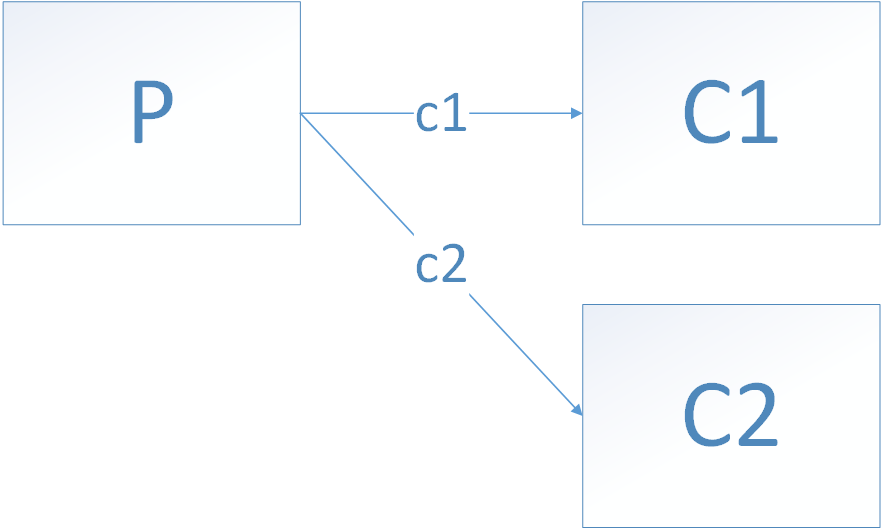
\includegraphics[width=10cm]{Images/00_Constraint_Schema}
	\end{frame}
	
	\begin{frame}
		\frametitle{Introduction}
		\framesubtitle{Rule Schema}
		\centering
		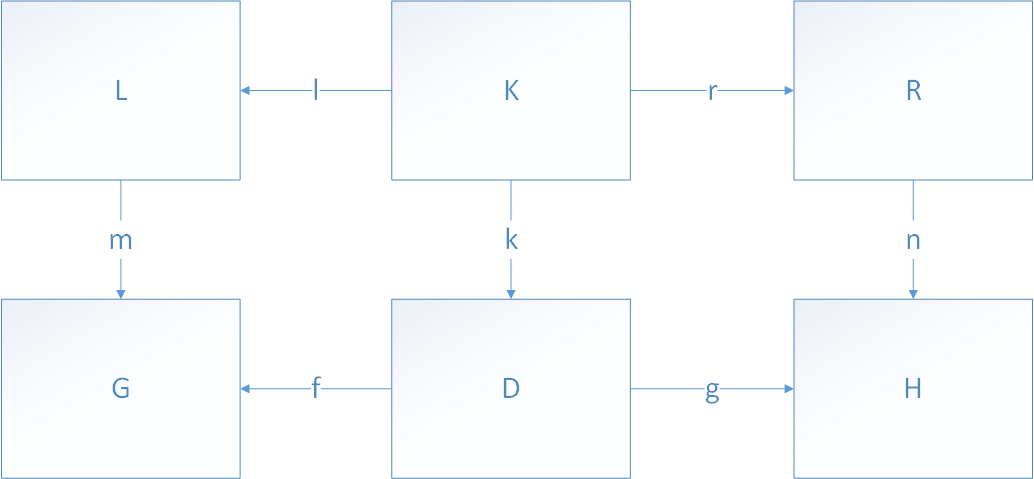
\includegraphics[width=12cm]{Images/00_Rule_Schema}
	\end{frame}

	\begin{frame}
		\frametitle{Introduction}
		\framesubtitle{Constraint Example}
		\centering
		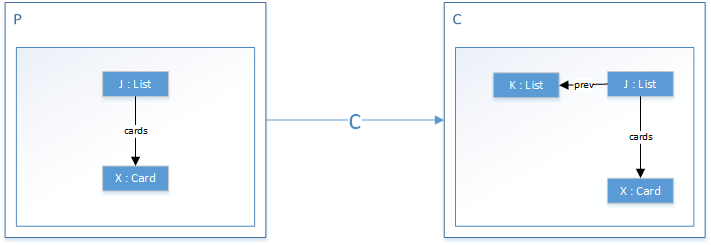
\includegraphics[width=12cm]{Images/01_Constraint_Example}
	\end{frame}

\section{Construction of Application Conditions from Constraints}
	\begin{frame}
		\frametitle{Contents}
		\tableofcontents[currentsection]
	\end{frame}

	\begin{frame}
		\frametitle{Construction of Application Conditions from Constraints}
		\framesubtitle{Construct $S$ -- Schema}
		\centering
		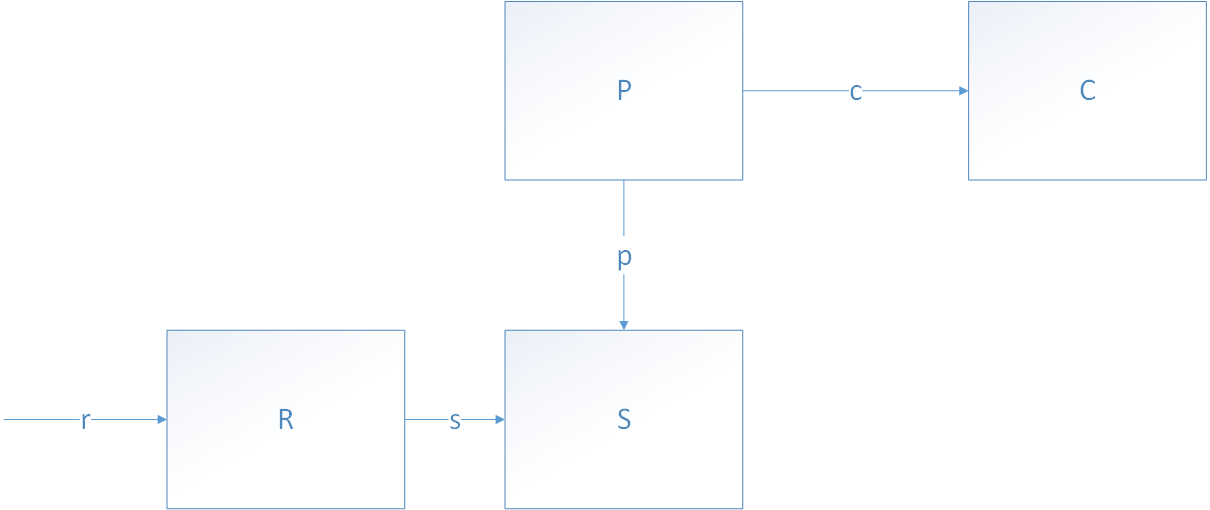
\includegraphics[width=12cm]{Images/10_Construct_S_Schema}
	\end{frame}

	\begin{frame}
		\frametitle{Construction of Application Conditions from Constraints}
		\framesubtitle{Construct $S$ -- Example Step 1}
		\centering
		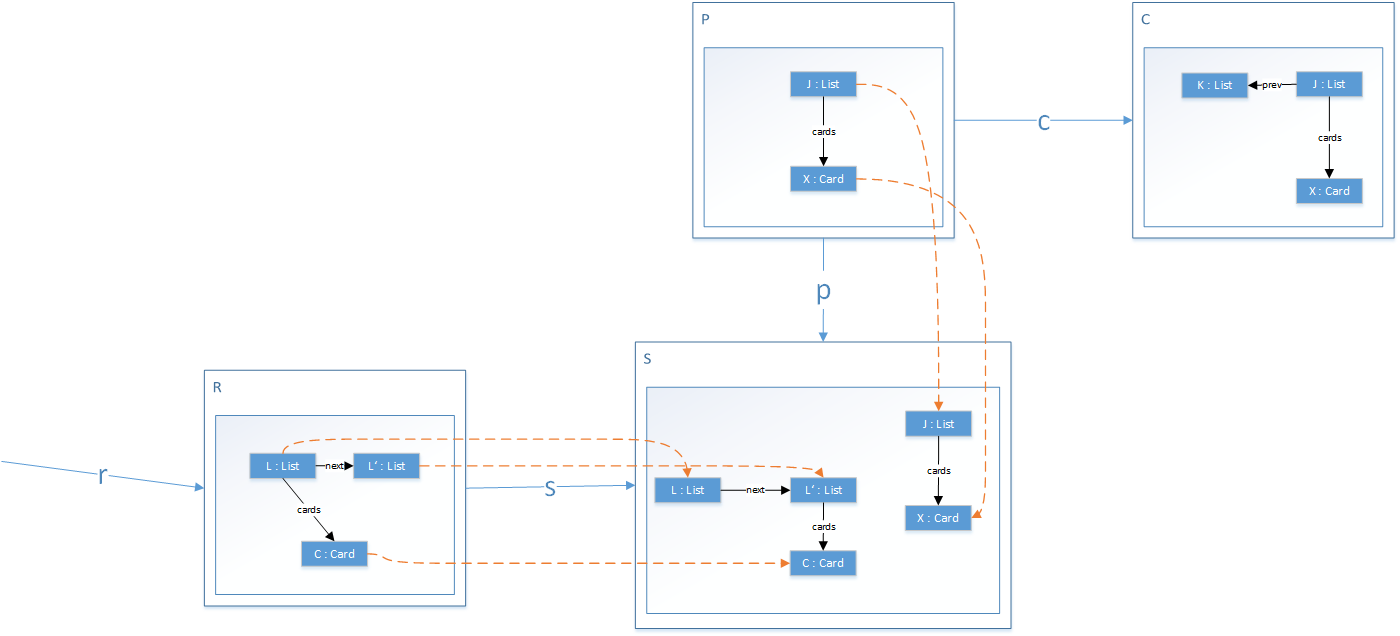
\includegraphics[width=12cm]{Images/11_Construct_S_Example_Step1}
	\end{frame}
	
	\begin{frame}
		\frametitle{Construction of Application Conditions from Constraints}
		\framesubtitle{Construct $S$ -- Example Step 2}
		\centering
		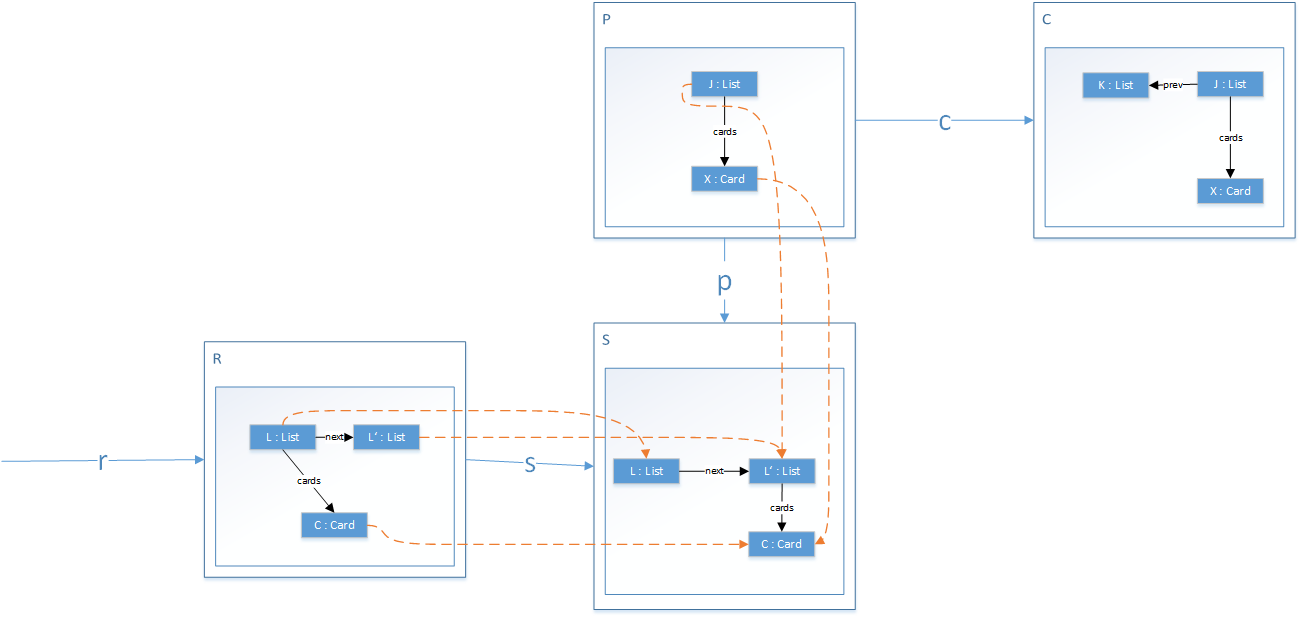
\includegraphics[width=12cm]{Images/12_Construct_S_Example_Step2}
	\end{frame}

	\begin{frame}
		\frametitle{Construction of Application Conditions from Constraints}
		\framesubtitle{Construct $T$ -- Schema}
		\centering
		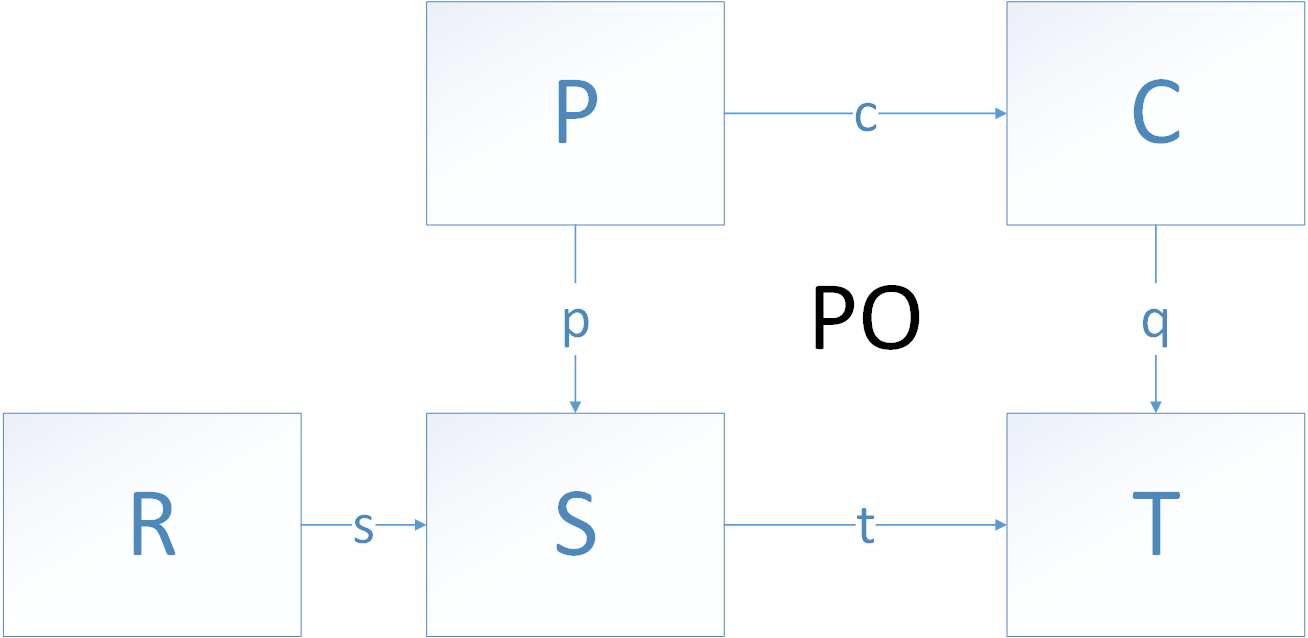
\includegraphics[width=12cm]{Images/20_Construct_T_Schema}
	\end{frame}

	\begin{frame}
		\frametitle{Construction of Application Conditions from Constraints}
		\framesubtitle{Construct $T$ -- Example}
		\centering
		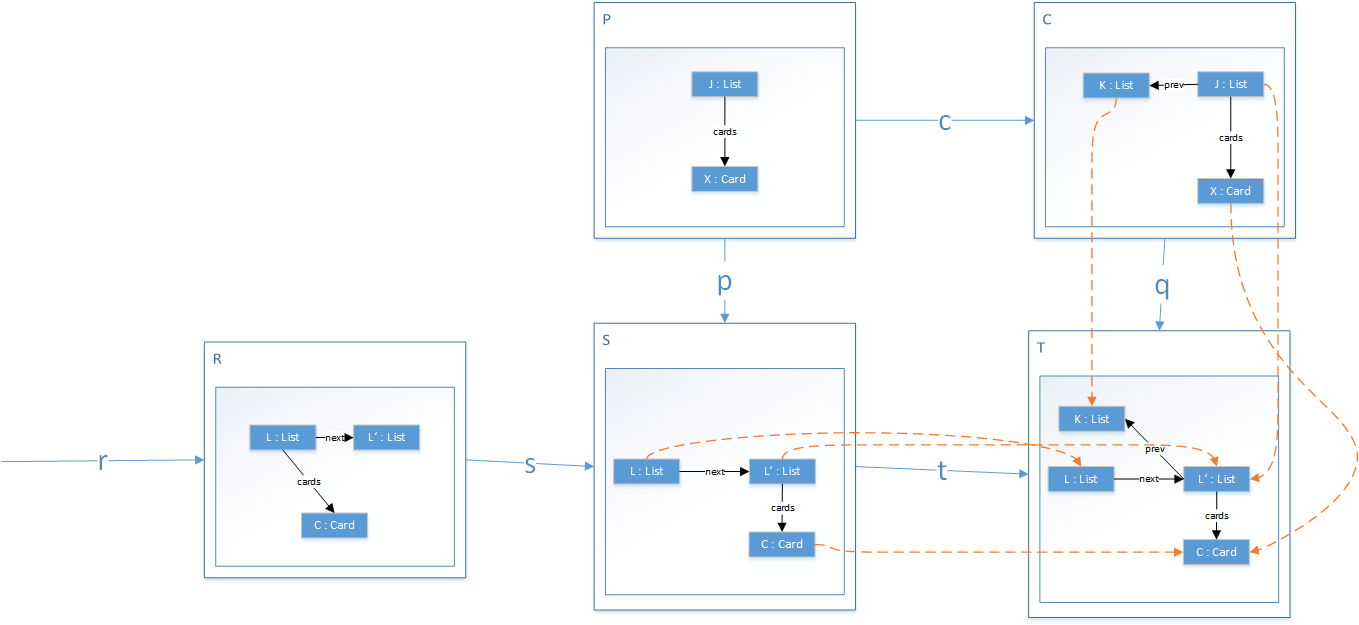
\includegraphics[width=12cm]{Images/21_Construct_T_Example}
	\end{frame}

	\begin{frame}
		\frametitle{Construction of Application Conditions from Constraints}
		\framesubtitle{Construct $T_i$ -- Schema}
		\centering
		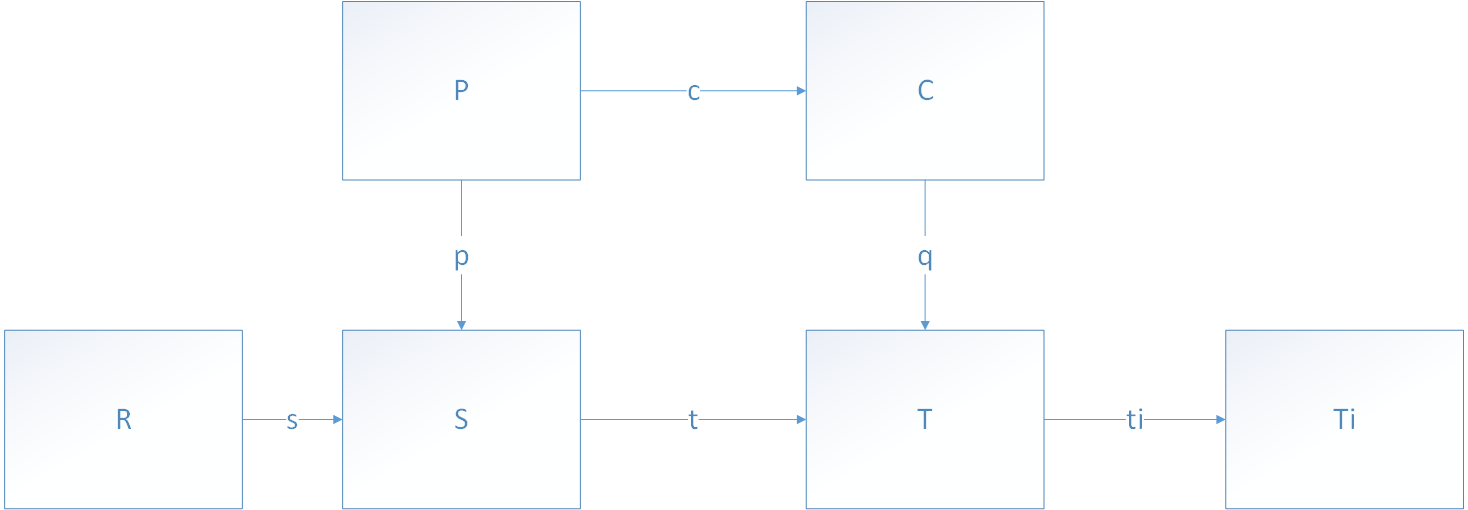
\includegraphics[width=12cm]{Images/30_Construct_Tis_Schema}
	\end{frame}

	\begin{frame}
		\frametitle{Construction of Application Conditions from Constraints}
		\framesubtitle{Construct $T_i$ -- Example}
		\centering
		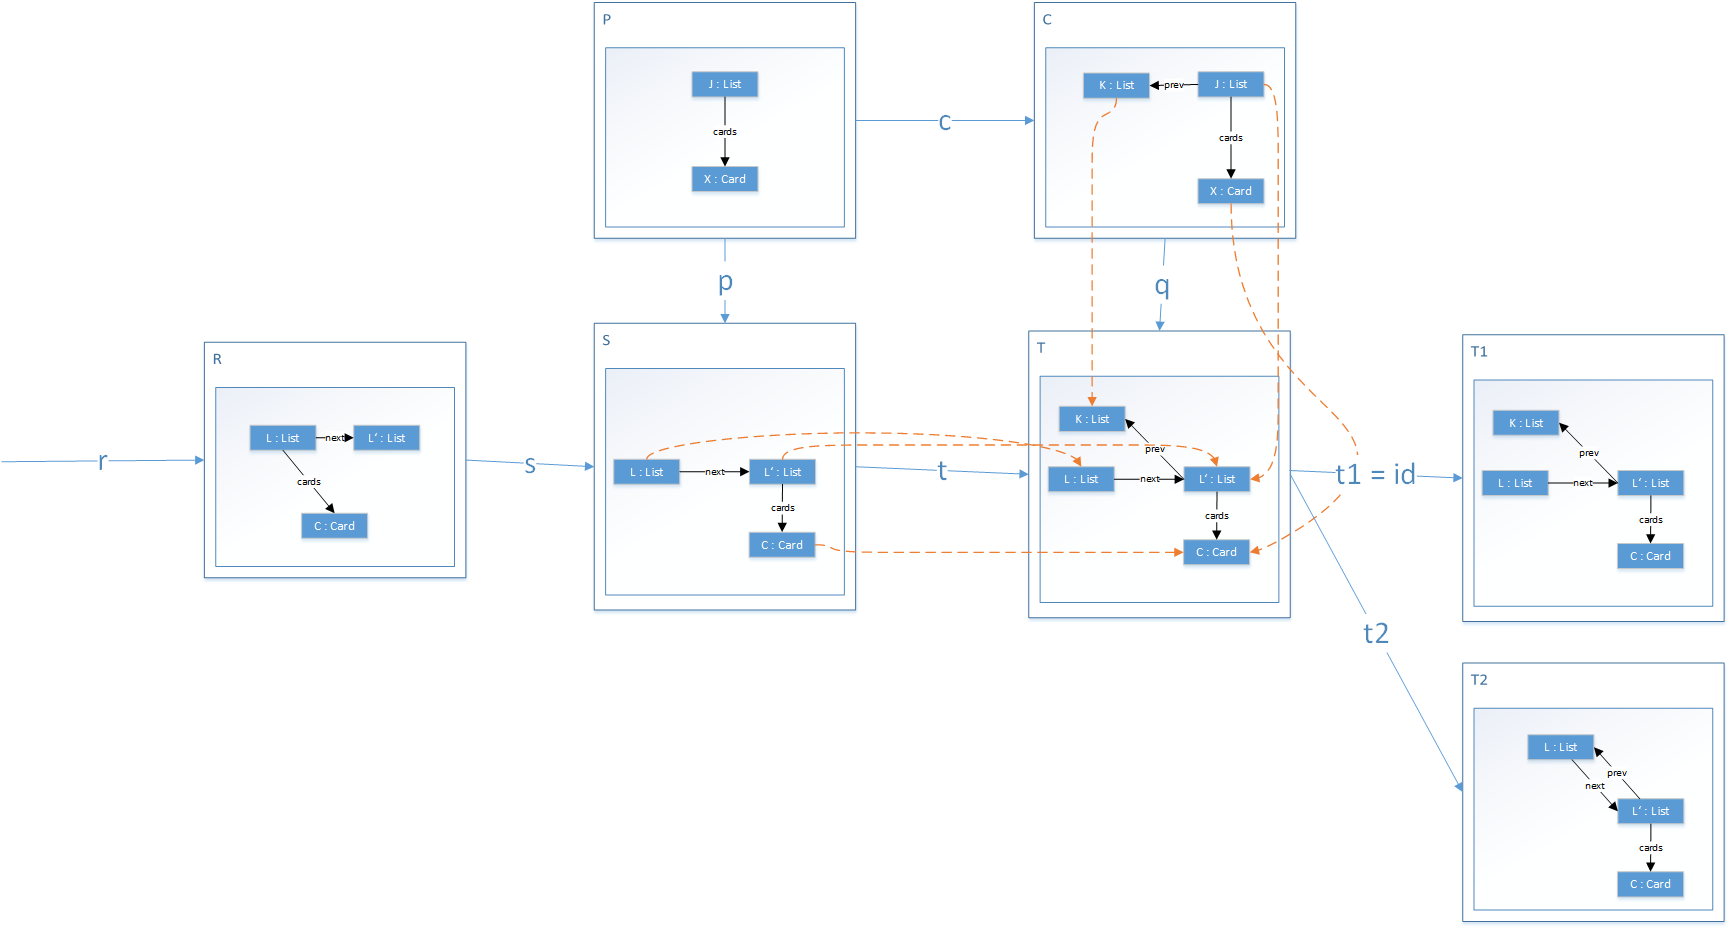
\includegraphics[width=12cm]{Images/31_Construct_Tis_Example}
	\end{frame}

\section{Construction of Left from Right Application Conditions}
	\begin{frame}
		\frametitle{Contents}
		\tableofcontents[currentsection]
	\end{frame}

	\begin{frame}
		\frametitle{Construction of Left from Right Application Conditions}
		\framesubtitle{Overview}
		\centering
		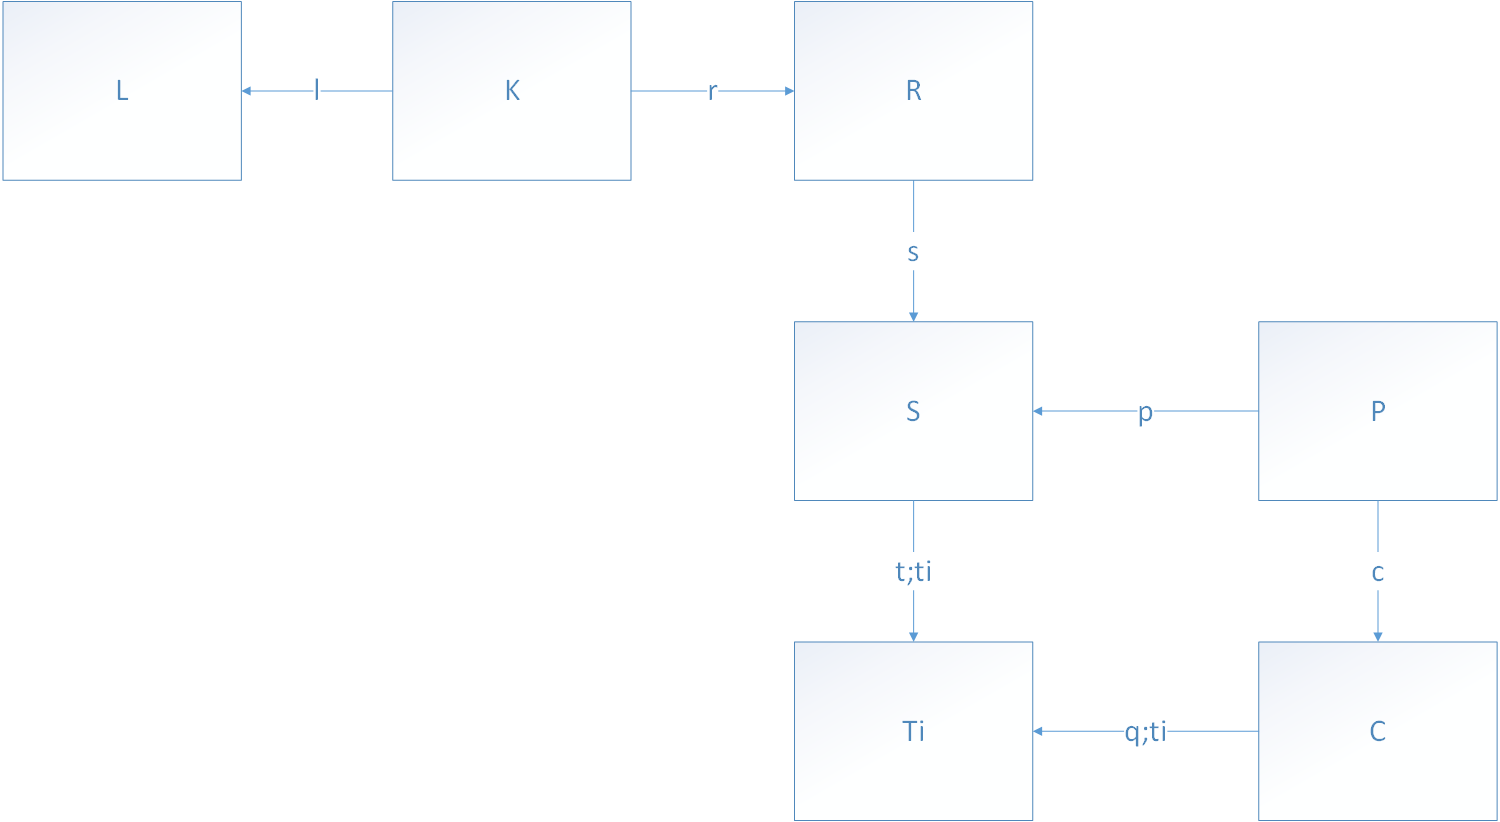
\includegraphics[width=12cm]{Images/40_Overview_RightAC_Schema}
	\end{frame}

	\begin{frame}
		\frametitle{Construction of Left from Right Application Conditions}
		\framesubtitle{From Right to Left Application Conditions -- Schema}
		\centering
		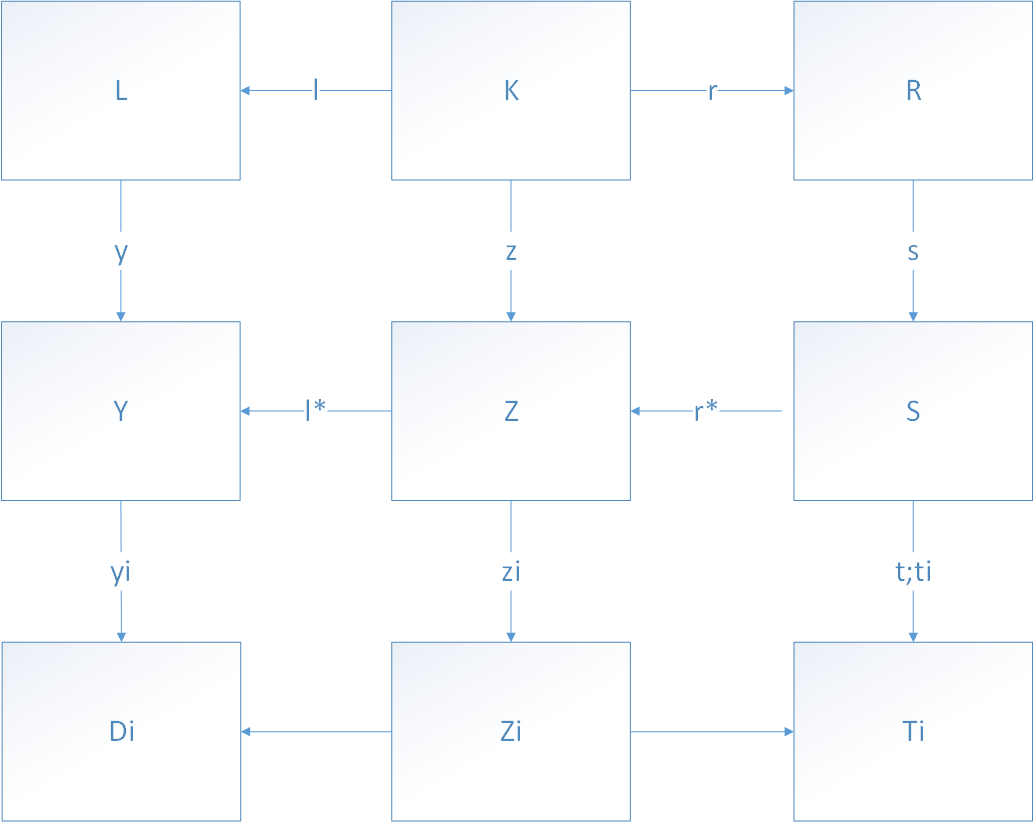
\includegraphics[width=9cm]{Images/50_RightAC-To-LeftAC_Schema}
	\end{frame}

	\begin{frame}
		\frametitle{Construction of Left from Right Application Conditions}
		\framesubtitle{From Right to Left Application Conditions -- Example Step 1}
		\centering
		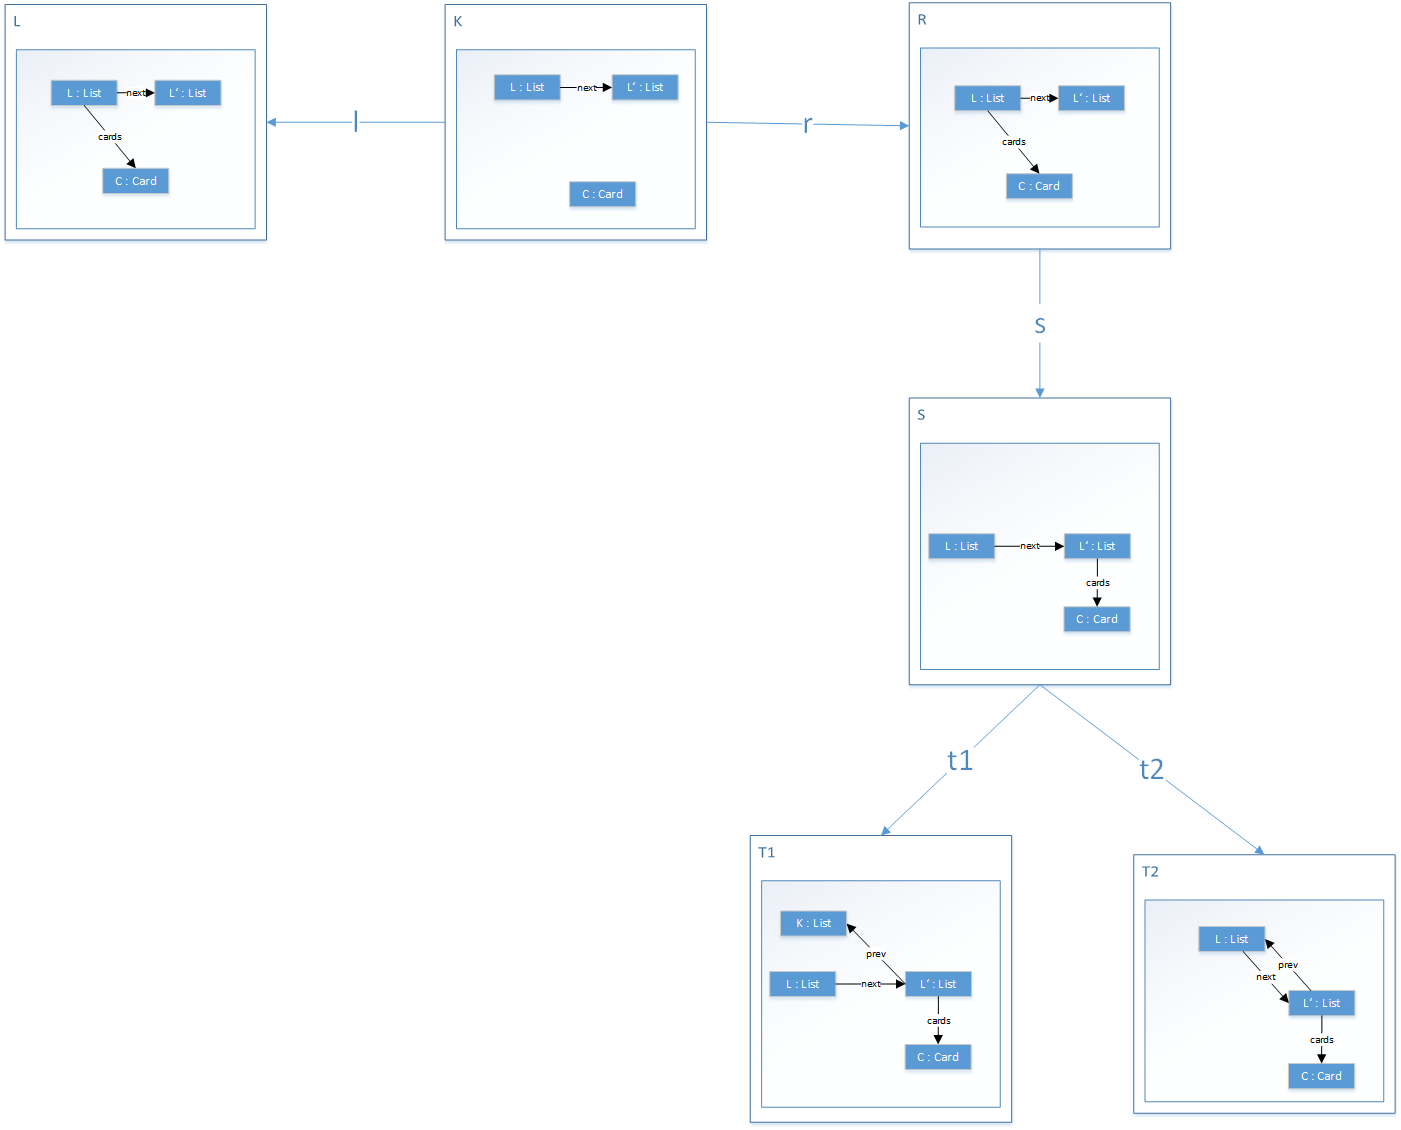
\includegraphics[width=9cm]{Images/51_RightAC-To-LeftAC_Example_Step1}
	\end{frame}
	
	\begin{frame}
		\frametitle{Construction of Left from Right Application Conditions}
		\framesubtitle{From Right to Left Application Conditions -- Example Step 2}
		\centering
		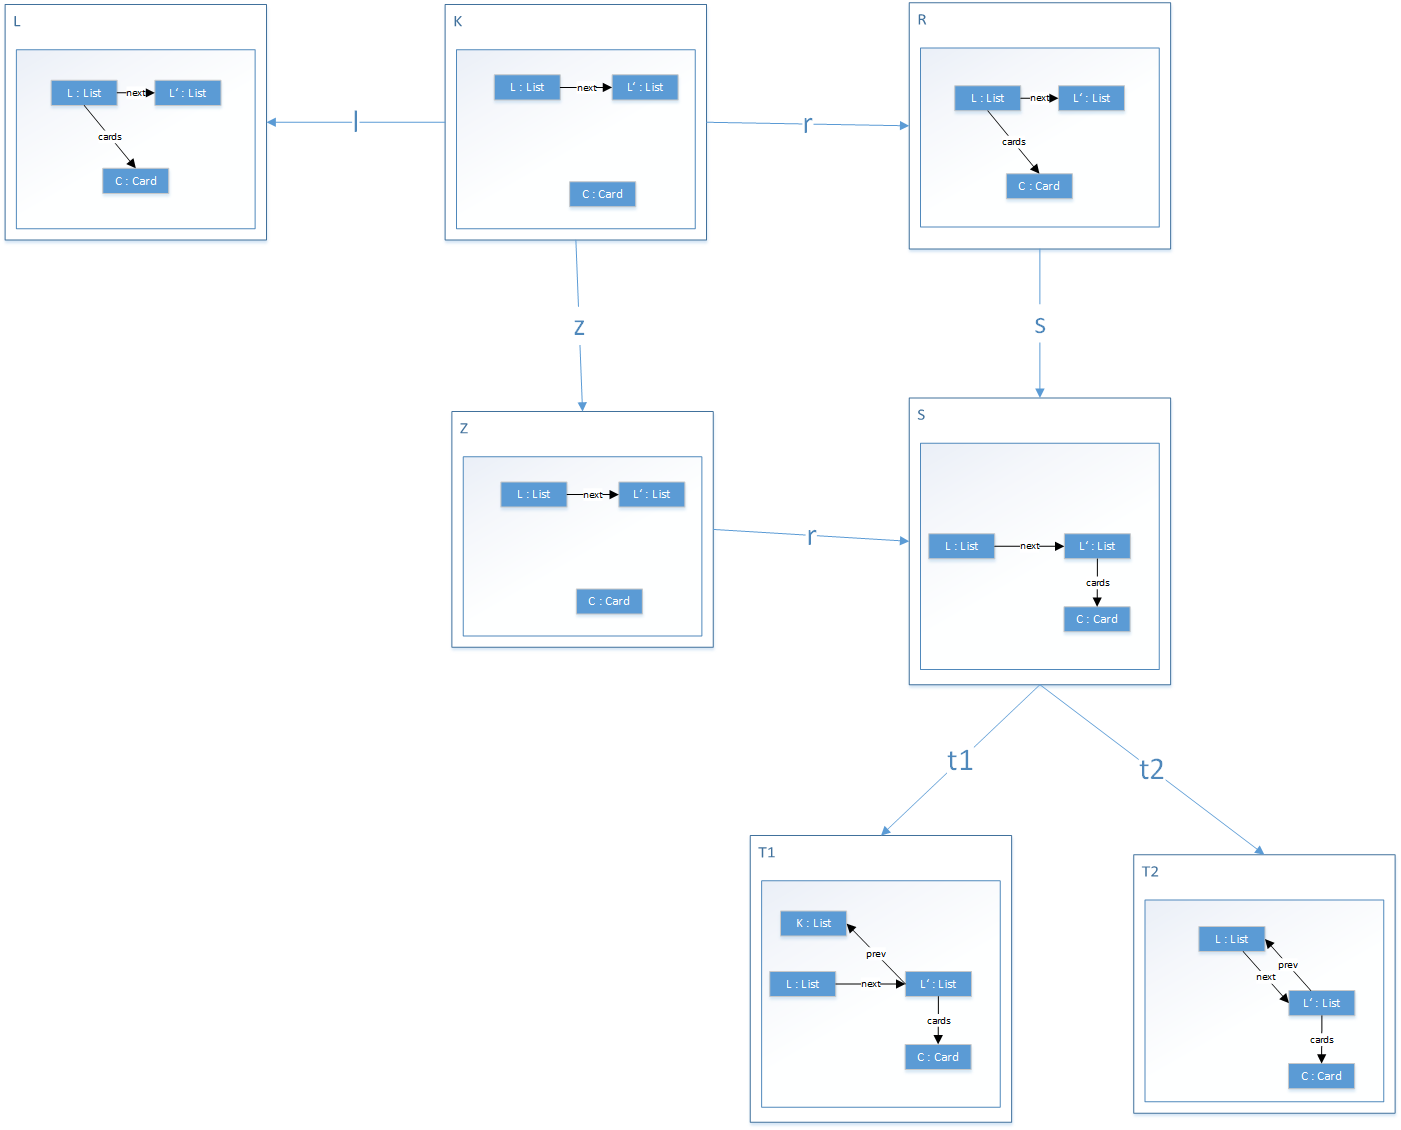
\includegraphics[width=9cm]{Images/52_RightAC-To-LeftAC_Example_Step2}
	\end{frame}

	\begin{frame}
		\frametitle{Construction of Left from Right Application Conditions}
		\framesubtitle{From Right to Left Application Conditions -- Example Step 3}
		\centering
		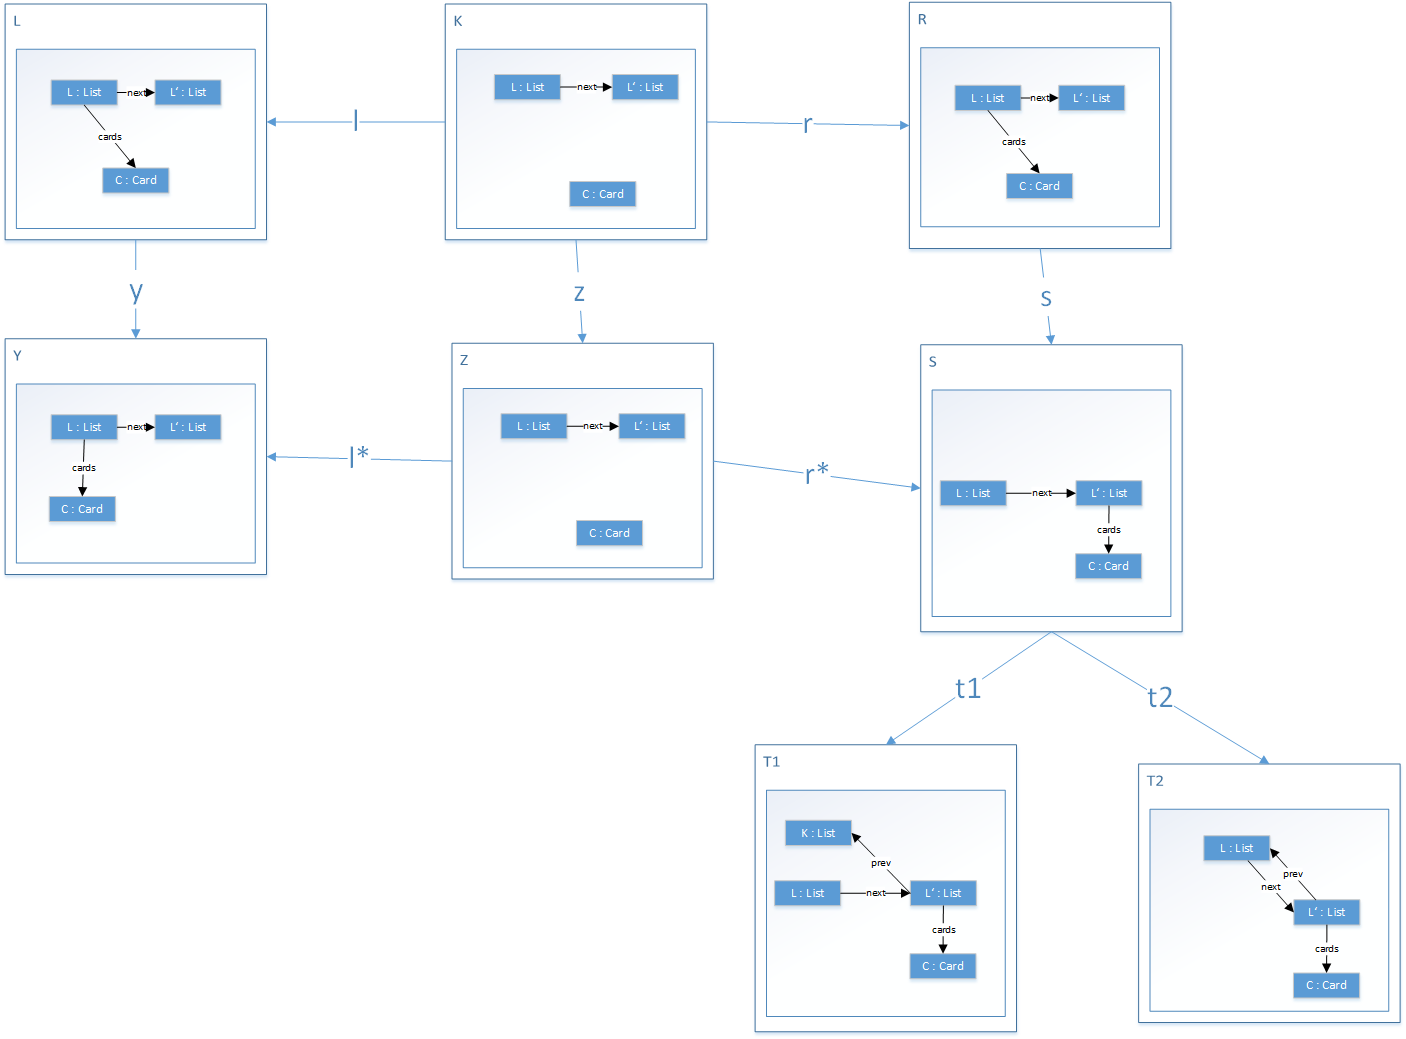
\includegraphics[width=9cm]{Images/53_RightAC-To-LeftAC_Example_Step3}
	\end{frame}

	\begin{frame}
		\frametitle{Construction of Left from Right Application Conditions}
		\framesubtitle{From Right to Left Application Conditions -- Example Step 4}
		\centering
		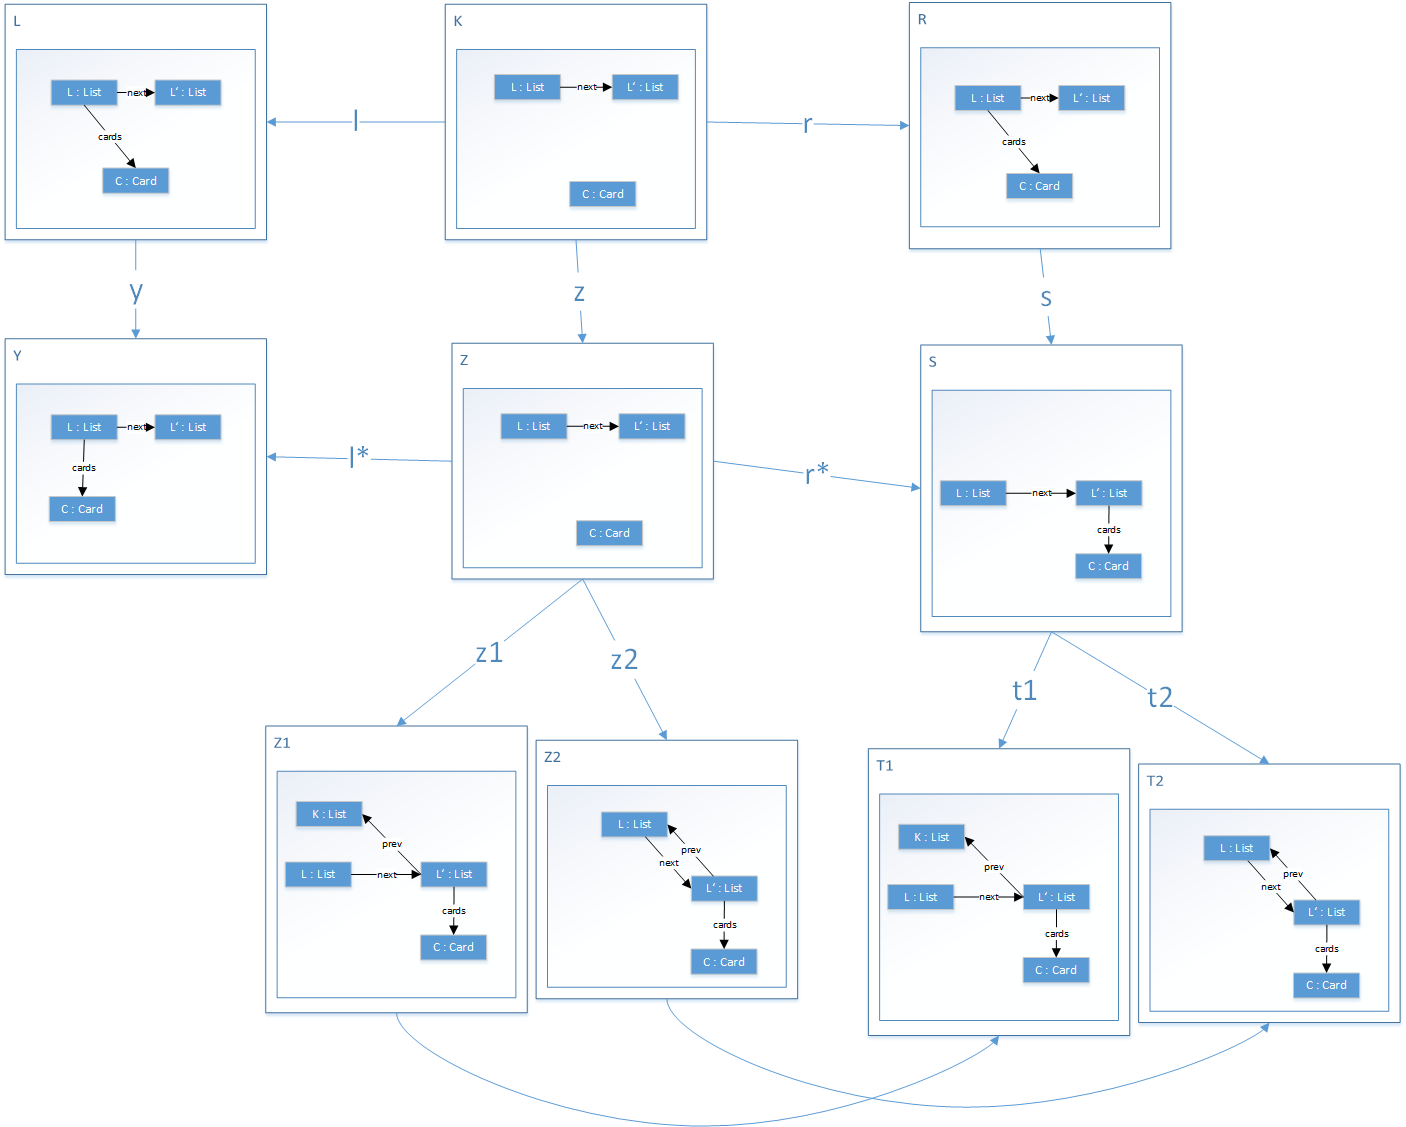
\includegraphics[width=9cm]{Images/54_RightAC-To-LeftAC_Example_Step4}
	\end{frame}

	\begin{frame}
		\frametitle{Construction of Left from Right Application Conditions}
		\framesubtitle{From Right to Left Application Conditions -- Example Step 5}
		\centering
		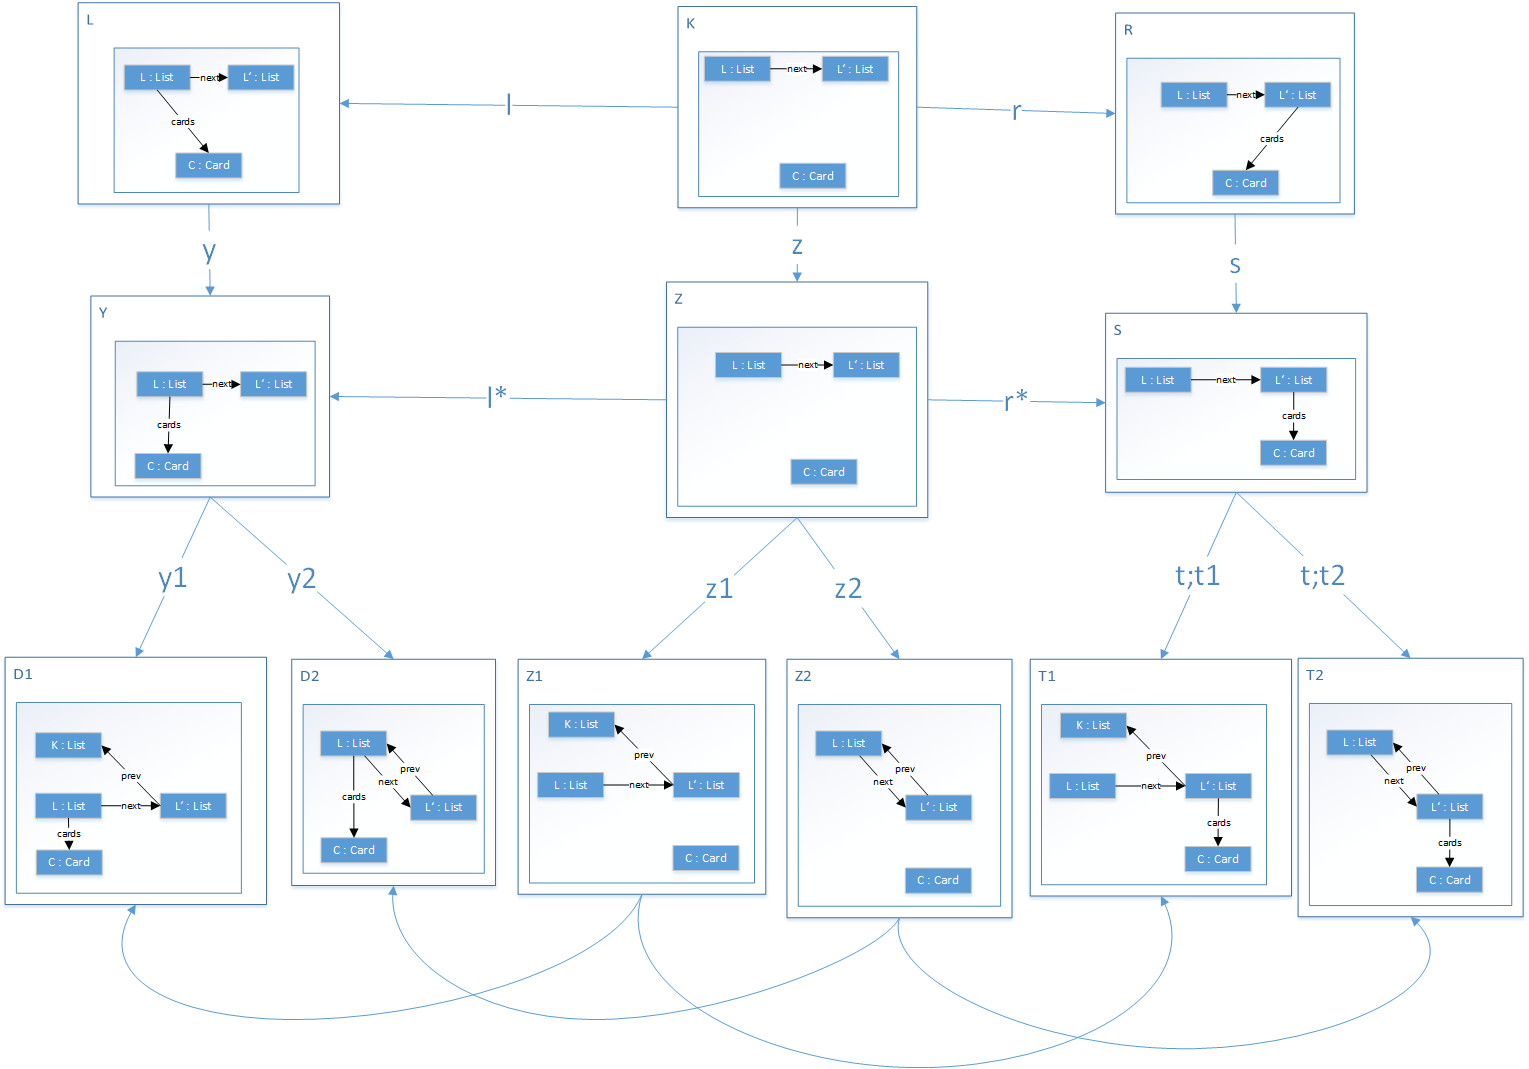
\includegraphics[width=10cm]{Images/55_RightAC-To-LeftAC_Example_Step5}
	\end{frame}

	\begin{frame}
		\frametitle{Construction of Left from Right Application Conditions}
		\framesubtitle{Left Application Condition -- Example}
		\centering
		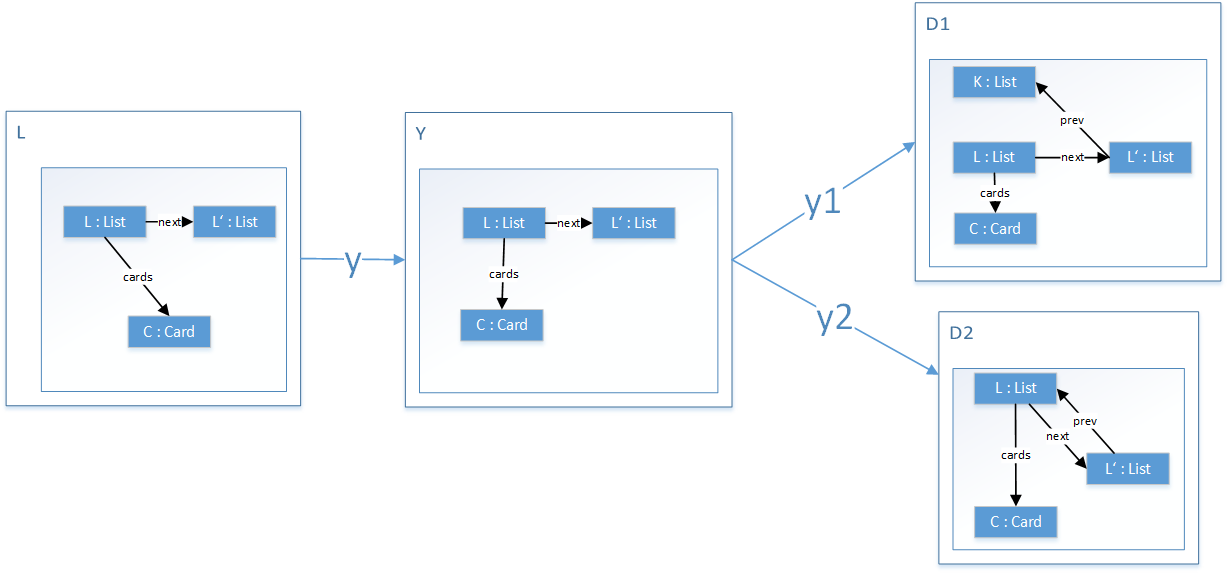
\includegraphics[width=12cm]{Images/60_Result-LeftAC}
	\end{frame}

\section{Lessions Learned}
	\begin{frame}
		\frametitle{Contents}
		\tableofcontents[currentsection]
	\end{frame}
	
	\begin{frame}
		\frametitle{Lessions Learned}
		\framesubtitle{}
		\begin{itemize}
			\item The construction of applications conditions can be implemented with the code from the exercises
			\item Problems:
				\begin{itemize}
					\item choose left or right and first or second in corners/spans?
					\item difficult to output diagrams in Plantuml as labels are used to identify objects in the diagrams (but there exist multiple objects with the same label) - no help for debugging  
				\end{itemize}
			\item Code generation for category theory would be great!
		\end{itemize}
	\end{frame}		
	
\end{document}